\documentclass[paper=A4]{article}
\usepackage{graphicx}
\begin{document}
	\section*{Notizen PMT}
	\subsection*{12.04.2021}
	Ziel Methoden und Techniken des Programmierens. \\
	im zweiten Teil Blick in den Speicher. \\
	Wiederholung Array: \\
	Array ist ein Speicherbereich (Vorstellung als Reihung) \\
	Array enthält Speicheradressen zu anderen Objekten. \\
	Klasse enthält Equal- get- und toStringmethode. GANZ wichtig!! \\
	Denke an generische Typen. \\
	Iterative Liste. \\
	Linked List \\
	Jedes Element kennt das nächste Element. \\
	Besonders schnelle Iteration. \\
	Schlecht um bestimmten Index zu suchen. \\
	Algorithmus Länge: \\
	Jedes Element gibt seine Länge + 1 aus. \\
	Algorithmus Contains: \\
	Jedes Element wird nacheinander geprüft ob es ein Element hat und ob das Element zur suche equals ist. \\
	Wenn die Prüfung fehlschlägt wird das Nachbarelement geprüft. \\
	For all: \\
	Jedes Element wird geprüft ob es leer ist und wenn nicht führt es die Anweisung aus und übergibt die Anweisung an das nächste Element. \\
	Beispiel für Implementierung der Samples s.o. \\
	RechteHand traditionell: head \\
	jeder head hat einen tail (Restliste). \\
	LL ist eine rekursive Liste \\
	AL it eine iterative Liste \\
	BoxPointerNotation \\
	\subsection*{15.03.2021}
	Def. Listen: \\
	Sei E eine Menge von Elementen. Die Menge der Listen über E. \\
	Sei List die kleinste Menge, für die gilt: \\
	1. Nil $\in$ List \\
	2. Wenn e $\in$ E xs $\in$ List, dann ist auch cons(e, xs) $\in$ List. \\
	Beachte Gleichungen für Realisierung der Rekursion. \\
	Erst überlegen: Endzustand \\
	Dann Überlegen: Folgezustand
	\subsection*{19.04.2021}
	Rede ans Volk bezüglich Motivation im Studium Sven Eric Panitz. \\
	Consumer und Lambdaausdruck \\
	Unterschiedliche Typen beachten. \\
	Eine Liste von Strings ist keine Liste von Objekten. \\
	verboten \\
	Parameter darf allgemeiner werden \\
	Rückgabe darf spezieller sein. \\
	\subsection*{22.04.2021}
	Def. Iteration - Wiederholen \\
	Beispiel am While Loop \\
	besser als ForLoop \\
	Loop hat Test, body, step \\
	Hinführung Implementierung von iterable \\
	Erstelle Objekt, dass test, body und step für Struktur implementiert und BAM Brudi, Schleife!! \\
	\subsection*{26.04.2021}
	Iteratoren über Listen \\
	definieren einer Schleife für bestimmte Klasse. \\
	Das Objekt soll mir sagen wie seine schleife geht. \\
	Interface iterable \\
	Schleife besteht immer aus test, body und step. \\
	hasNext = test \\
	Next = body und step \\
	Iterator implementiert Schleifenkopf!!! \\
	\subsection*{29.04.2021}
	iterable \\
	iterierbare Objekte \\
	einfaches Beispiel für count mit foreach  \\
	Summe \\
	Einstieg für Faltung da Summe nur CopyPaste von Count \\
	Faltungen \\
	Typ wird variabel \\
	Falte eine Iteration zu einer Einziegen Antwort zusammen.
	java.util.stream für Faltungen hat nix zutun mit IO. \\
	\subsection*{03.05.2021}
	Faltungen \\
	häufige Schleife \\
	Auf eine Ergebnisvariable wird immer wieder etwas aufaddiert in jedem Penetrationsvorgang \\
	Streams, Spliterator \\
	Stream \\
	- Erzeugen: z.B. of \\
	- Modifikation: z.B. parallel \\
	- Verbrauch: collect, reduce, foreach \\
	Streams Einmalobjekt \\
	nach Iteration neu erzeugen \\
	Verbrauchende Funktionen: ForEach, \\
	Stream(objekt) \\
	Menge hat zwei Implementierungen \\
	 treeset, hashset
	\subsection*{06.05.2021}
	Spliterator \\
	Iterator hasNext und Next \\
	Stream verwendet Spliterator \\
	arbeiten parallel \\
	Spliteratoren verwenden tryAdvance und vereinen hasNext und Next  \\
	Realisiert Iteration über Splititerator \\
	TryAdvance hat Consumer mit funktionalem Interface \\
	Nur Methode TryAdvance ist wichtig. \\
	gibt boolean zurück, bekommt als Parameter einen Consumer  \\
	trySplit() teilt die Arbeit bei Spliteratoren die Partioniert werden können  \\
	trySplit Parallelisiert \\
	Beispiel Array: Aufteilung entlang der Länge \\
	Es gibt immer das This-Objekt und das neue Splitterobjekt
	\subsection*{10.05.2021}
	Bäume \\
	Weg von Liste zu Baum \\
	nicht nur ein tail sondern viele \\
	Baum hat Wurzel und eine Liste von Tails \\
	0 - beliebig viele tails \\
	rename tails to child \\
	Baum Schleife über Kinder jedes Kind hat viele Kinder  \\
	Bei ToString StringBuffer verwenden weil quadratischer Aufwand \\
	\subsection*{17.05.2021}
	Bäume mit Aussagenlogic wie in Semester 1. \\
	XML \\
	beschreibt Baumstrukturen \\
	Baumstruktur für XML \\
	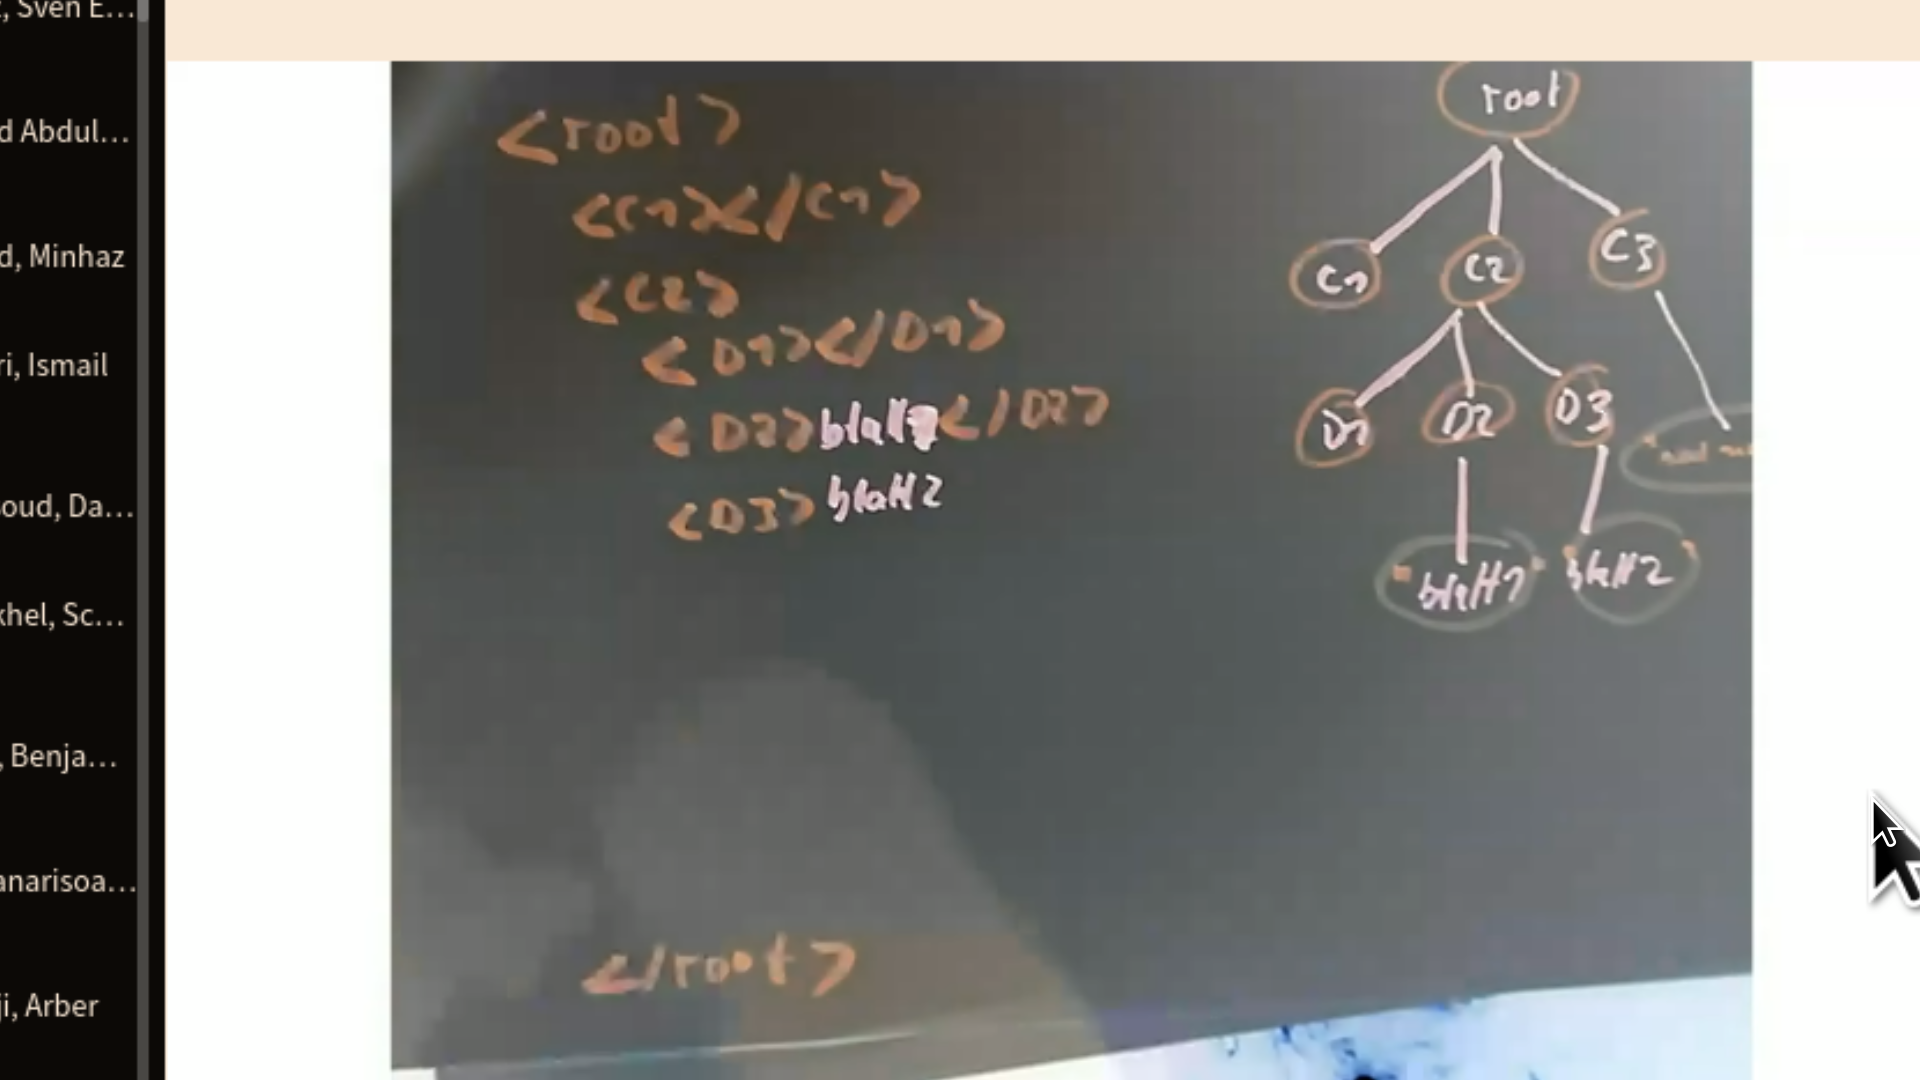
\includegraphics[width=\linewidth]{picbaum}
	Elementknoten \\
	Unterschiede zu HTMl: in HTML sind Elementknoten ganz genau festgelegt. \\
	XML erlaubt einfügen eigener Tags. \\
	XML ist immer ein Baum. \\
	bei XML müssen vor einem zu schließenden Tag alle darin geöffneten Tags geschlossen werden. \\
	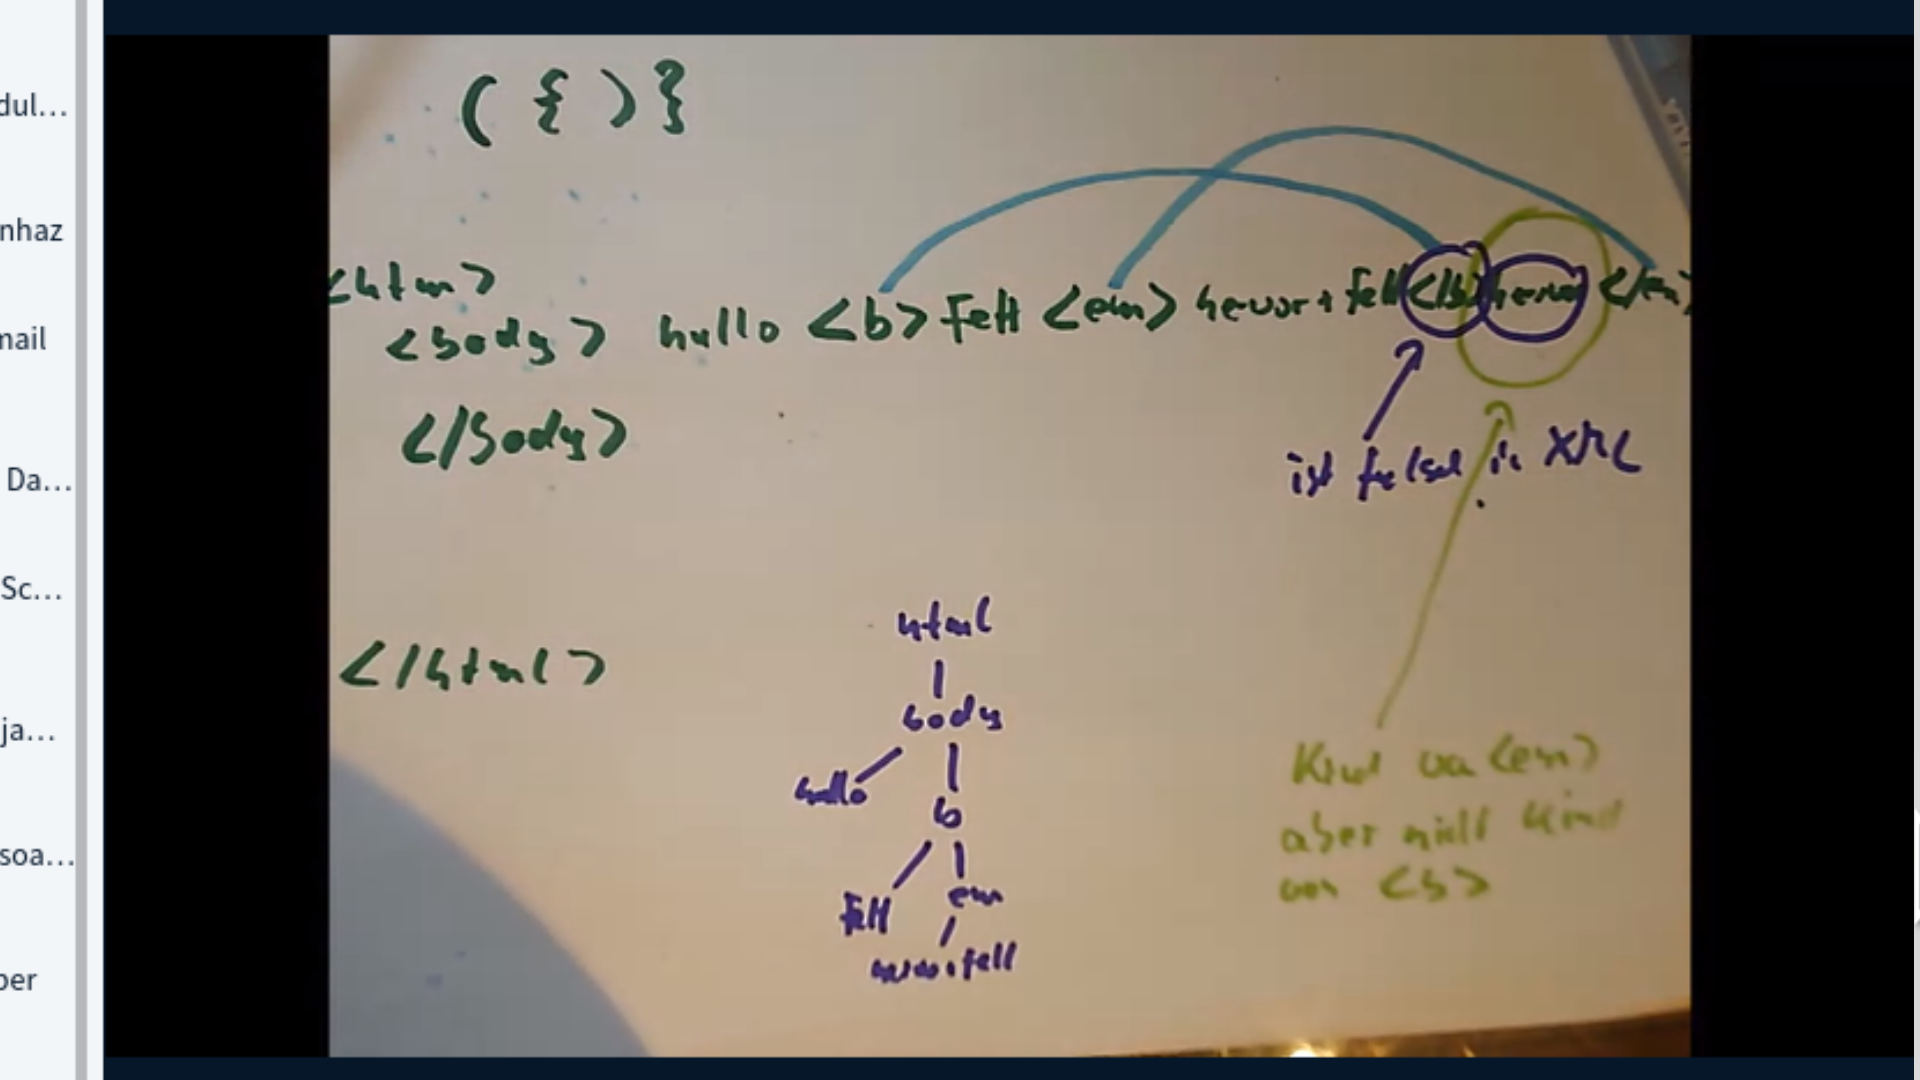
\includegraphics[width=\linewidth]{picbaum2} \\
	XML eindeutiger Knoten, im Knoten sollte Koodierung enthalten. \\
	XML kann Unicode. \\
	UTF-8 ist Standard \\
	SVG Daten \\
	clash in XML \\
	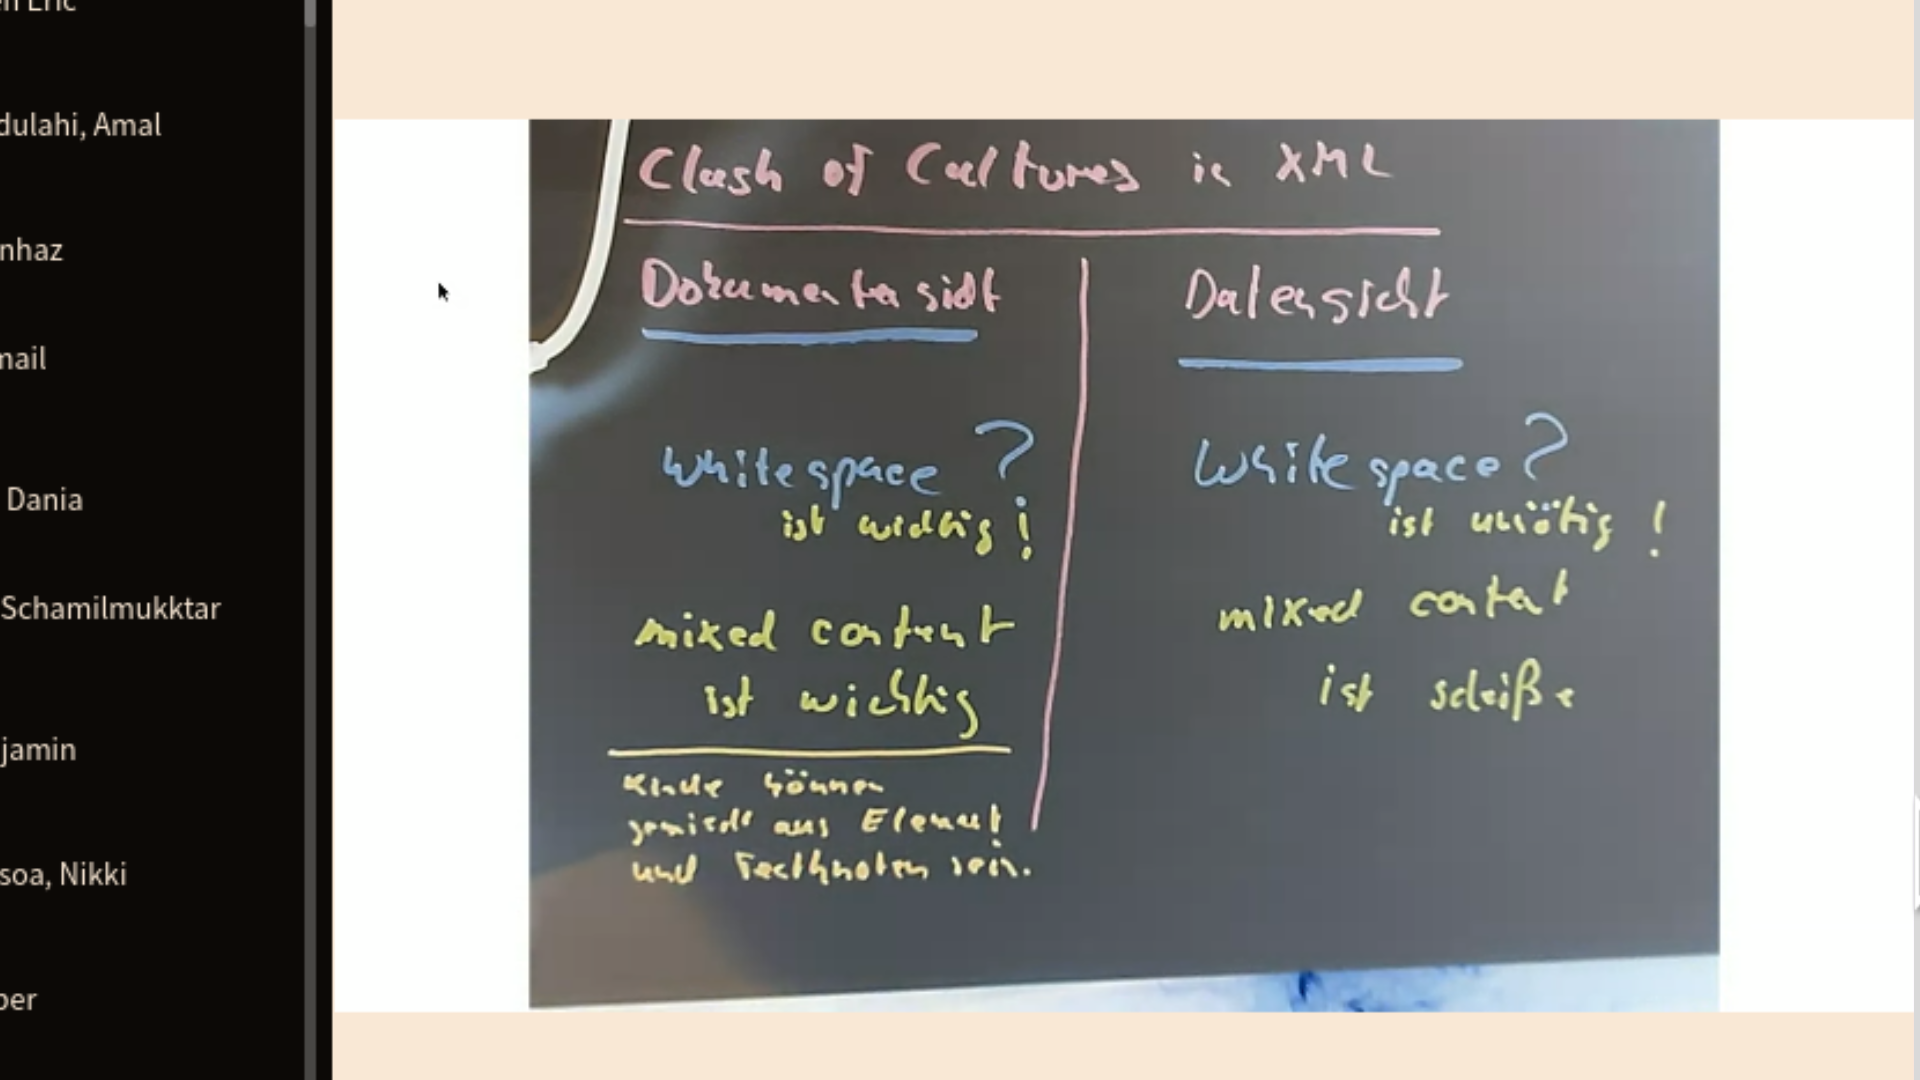
\includegraphics[width=\linewidth]{xmld} \\
	\subsection*{20.05.2021}
	Kommentarknoten \\
	jeder XML-Tag muss geschlossen werden.  \\ 
	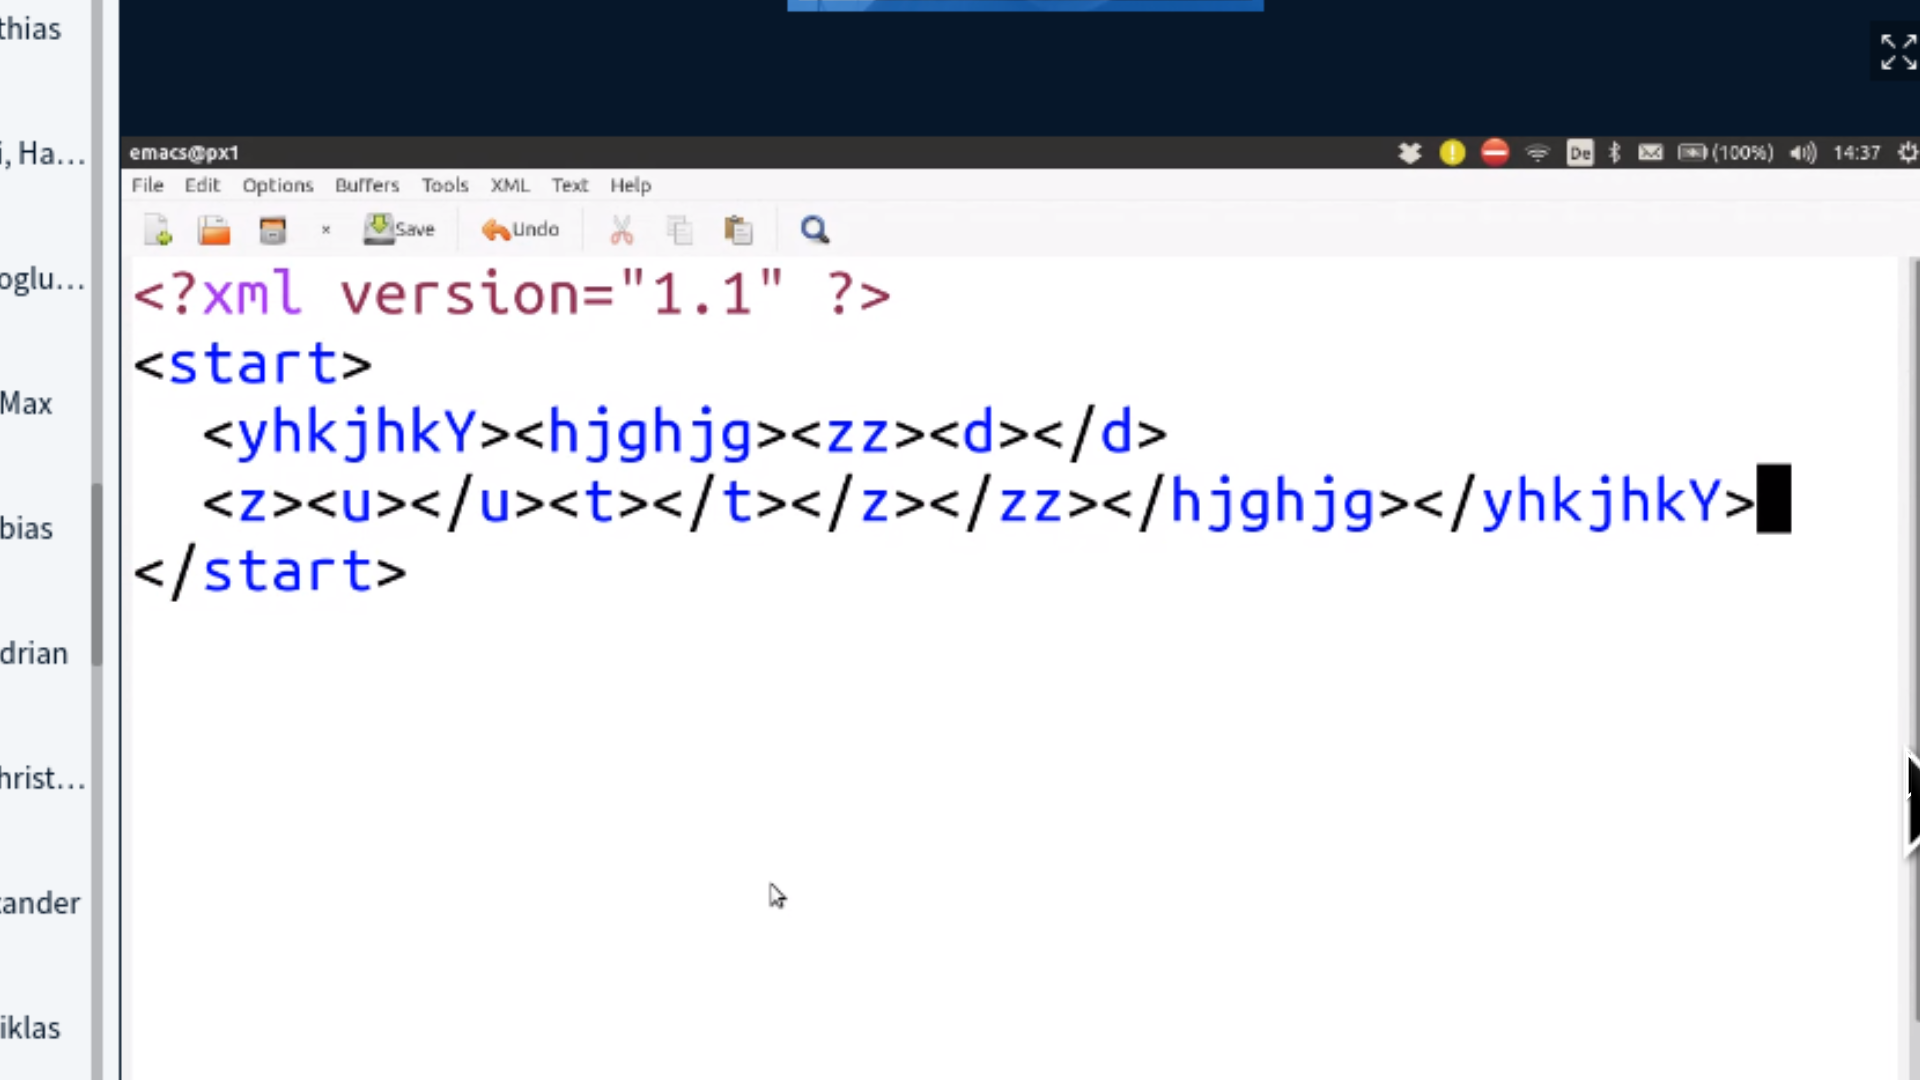
\includegraphics[width=\linewidth]{xmlsample}
	zeichen $<$ oder $>$ sind reserviert. \\
	Können mit Excapes trotzdem erzeugt werden. \\
	CDATA \\
	Tag Deklaration beginnt mit $<$ und endet mit $>$
	\\
	Innerhalb Öffnungstag Attribute möglich. \\
	Attribute hier als Menge von Schlüsselwertpaaren \\
	Schlüsselwertpaare = MAP \\
	XML hohe Syntaktische Strene \\
	hashmap Entryset \\
	\subsection*{27.05.2021}
	Knoten in XML, Text oder Map \\
	XML wurde unabhängig von einer Programmiersprache definiert. \\
	low level Programmierung \\
	XML API \\
	XML API besteht aus Interfaces \\
	wichtigstes Interface Note \\
	Parser für XML benutzen  \\
	Documentbuilderfactory \\
	Dokumentation: https://docs.oracle.com/javase/7/docs/api/org/xml/sax/SAXException.html \\
	Achsen \\
	\subsection*{31.05.2021}
	Dom ist ein API, dass unabhängig von Programmiersprachen entwickelt wurde. \\
	XPath W3C \\
	XPath Achsen \\
 	Def für Knoten im Baum sehr ausführlich. \\
 	XPath nie alleine wird von anderen Sprachen verwendet. \\
 	Xquery 	 \\
 	XML basierte Datenbanken \\
 	XSL ist xml dokument verarbeitet XML zu XML-Dokument \\
 	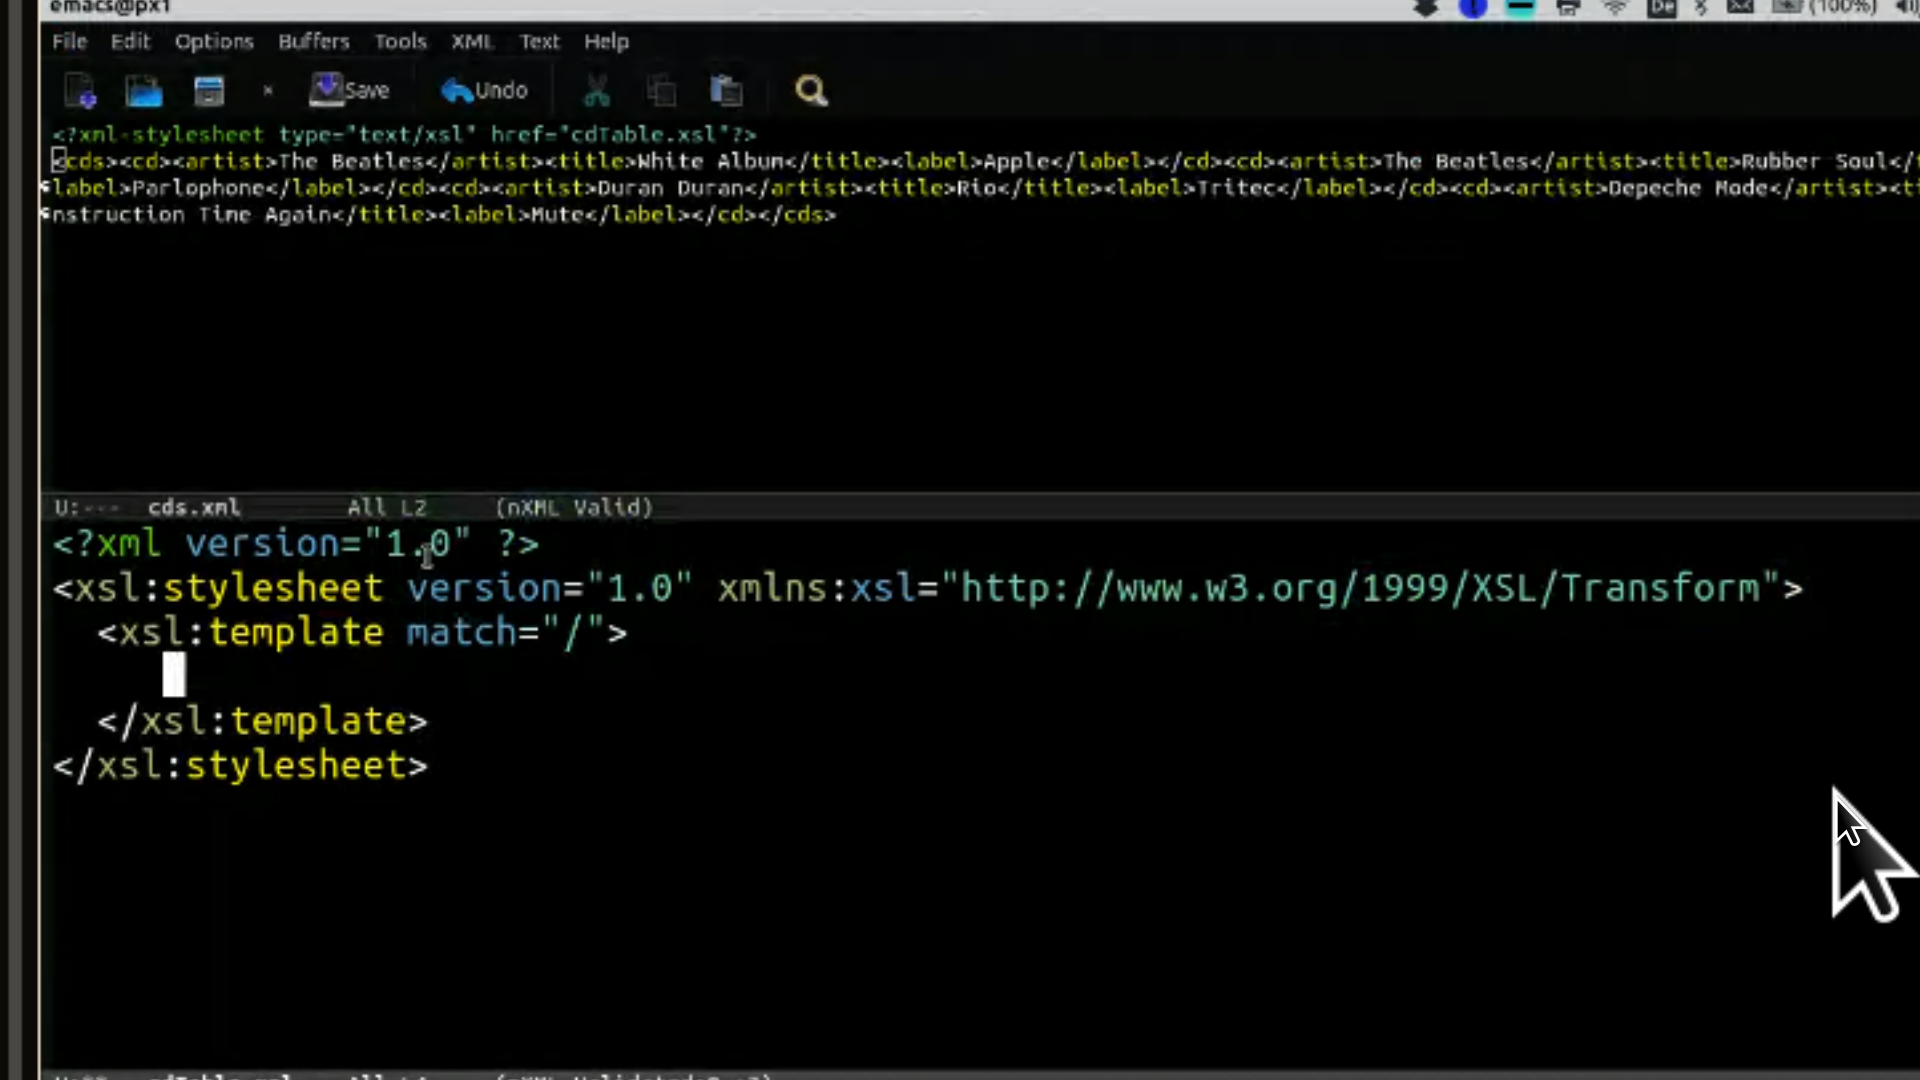
\includegraphics[width=\linewidth]{xslsample} \\
 	Beispiel für XSL aus der Vorlesung \\
 	XSL ist deklarativ. \\
 	SVG \\
 	Simple API for XML Processing \\
 	SAX \\
 	möglichst einfach und nah an der Praxis. \\
 	SAX durchläuft Dokument vollständig und kann bei bestimmten Ereignissen getriggert werden. \\
 	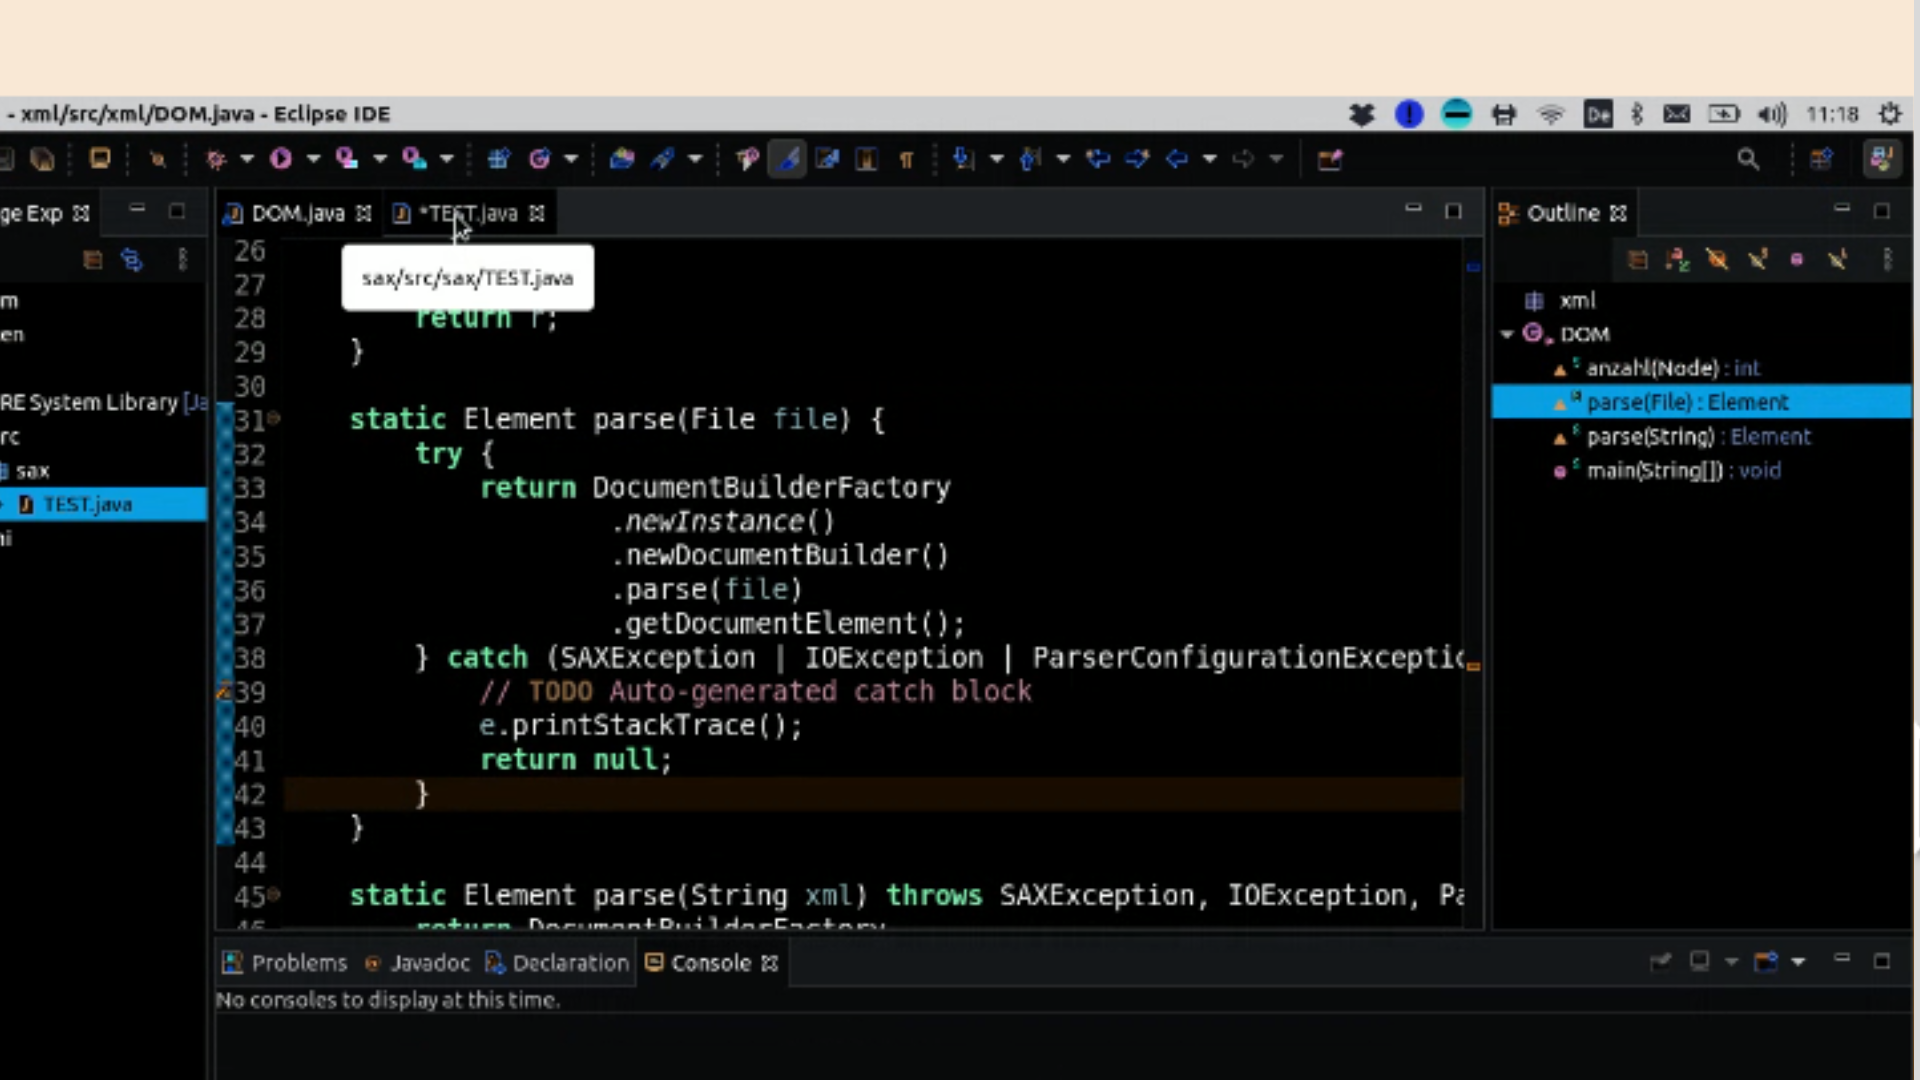
\includegraphics[width=\linewidth]{domparser}
 	Parser für DomAPI \\
 	Vorteil: Nie gesamtes Dokument im Speicher. \\
 	Nachteil: Kein Zugriff auf die Baumstruktur des XML Dokuments \\
 	\subsection*{07.06.2021}
 	Parser erzeugt syntaxbaum \\
 	Beispiele Java 17  \\
 	Switchcase über Paare \\
 	Document Type Definition \\
 	DTD \\
 	Teil von XML \\
 	DTD beschreibt außerhalb von XML Tags und deren erlaubte Kinder. \\
 	DTD legt Regeln für XML fest. \\
 	JSON JavaScriptObjectNotation \\
 	JavaScript \\
 	Jsonobjekt ist ein Map \\
 	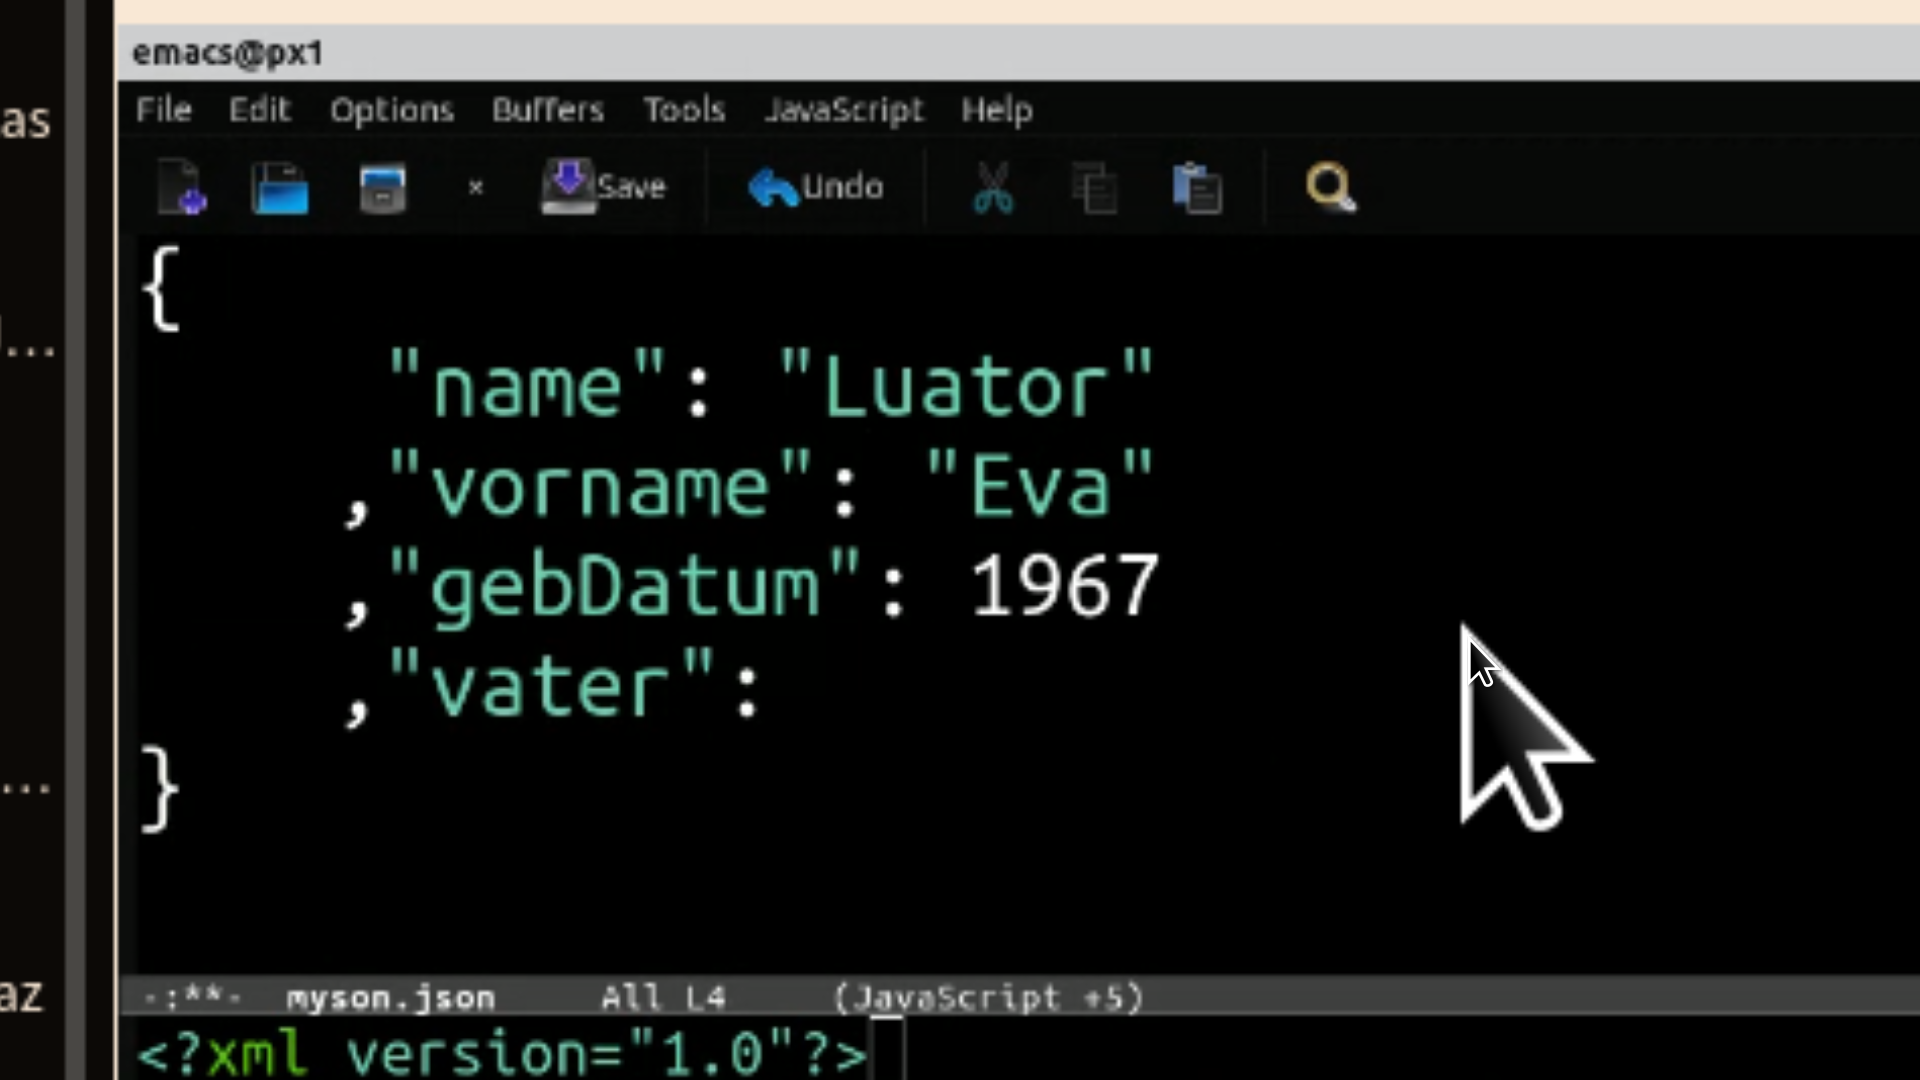
\includegraphics[width=\linewidth]{jsonsample} \\
 	\subsection*{10.06.2021}
 	Programmierung in C \\
 	C ähnelt sehr stark Java \\
 	main methode in C gibt int zurück. \\
 	C hat einen Siinlge parse compile.
 	Jede Information die notwendig ist muss bereits bekannt sein. \\
 	gcc -c Objekterstellung  \\
 	gcc compile und ausführen \\
 	.h definiert includes \\
 	Bekanntmachung \\
 	C kennt keine Methodenüberladung\\
 	In C keine Klassen, Strukturierung nur mit struct \\
 	Definition endet mit Semikolon.   \\
 	C lebt direkt im Arbeitsspeicher \\
 	C ist gaaaaaanz nah am System \\
 	\subsection*{14.06.2021}
 	Speicheralokkierung in C \\
 	Muss von Hand erledigt werden. \\
 	Stack \\
 	Speicherbereich im Hauptspeicher \\
 	Arbeitsbereich von oben auflegen und von oben herunternehmen \\
 	nach return sind alle lokalen Variablen weg.
 	Nur das Ergebnis einer Funktion bleibt.
 	heap \\
 	durchnummerierte Speicherzellen \\
 	Das Programm muss gespeichert werden
 	Programmspeicher \\
 	In C für den Heap selber verantwortlich \\
 	neues Objekt = Eintrag im Heap \\
 	in Java automatisch in C von Hand \\
 	h Datei bietet Methodensignaturen und sturkturierte Daten \\
 	* hat in C drei Bedeutungen: \\
 	1. Teil der Typsignatur \\
 	2. Vor unären Operator: Adresse auf Speicherzelle\\
 	Dereferenzieren. \\
 	3. Multiplikation \\
 	Speicher auf dem Heap holen mit malloc(Größe in Byte) \\
 	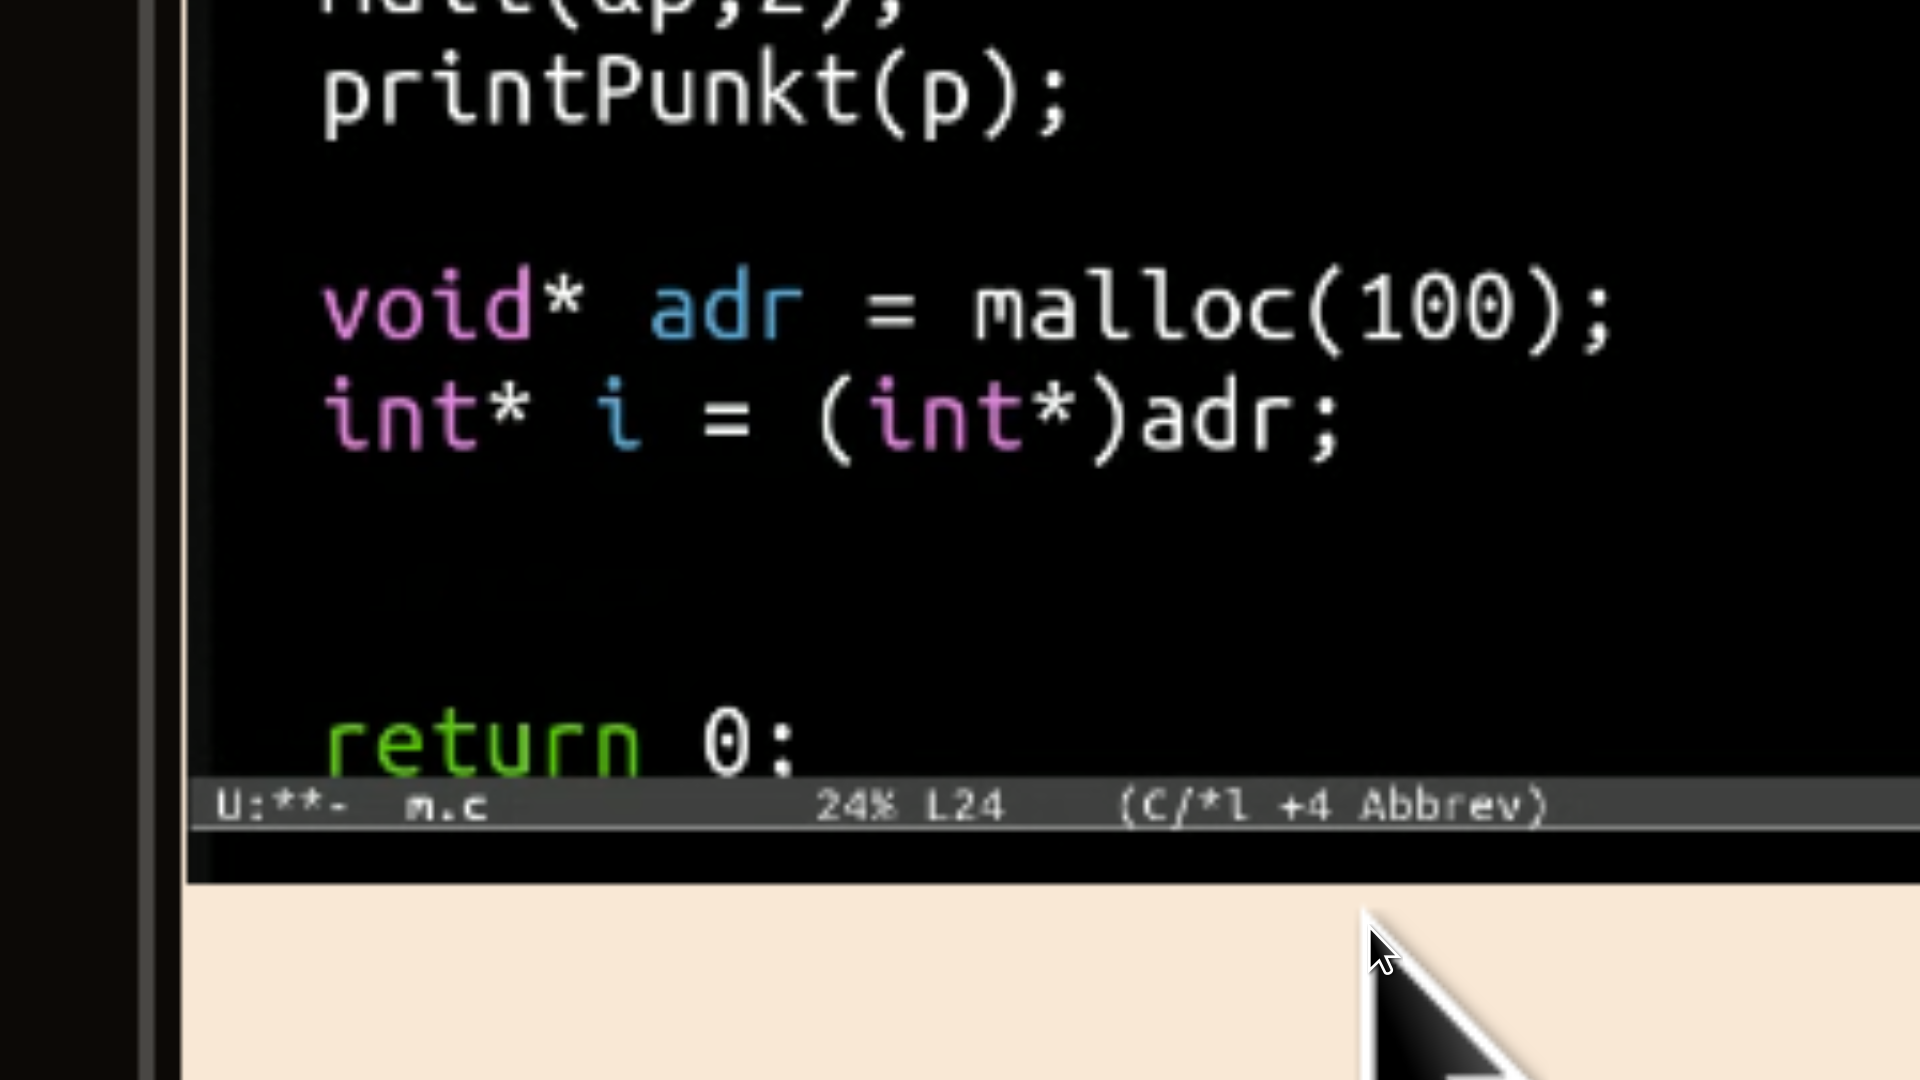
\includegraphics[width=\linewidth]{samplec}
 	\\
 	\subsection*{17.06.2021}
 	malloc() Speicherbelegung in Byte aUF DEM Heap. \\
 	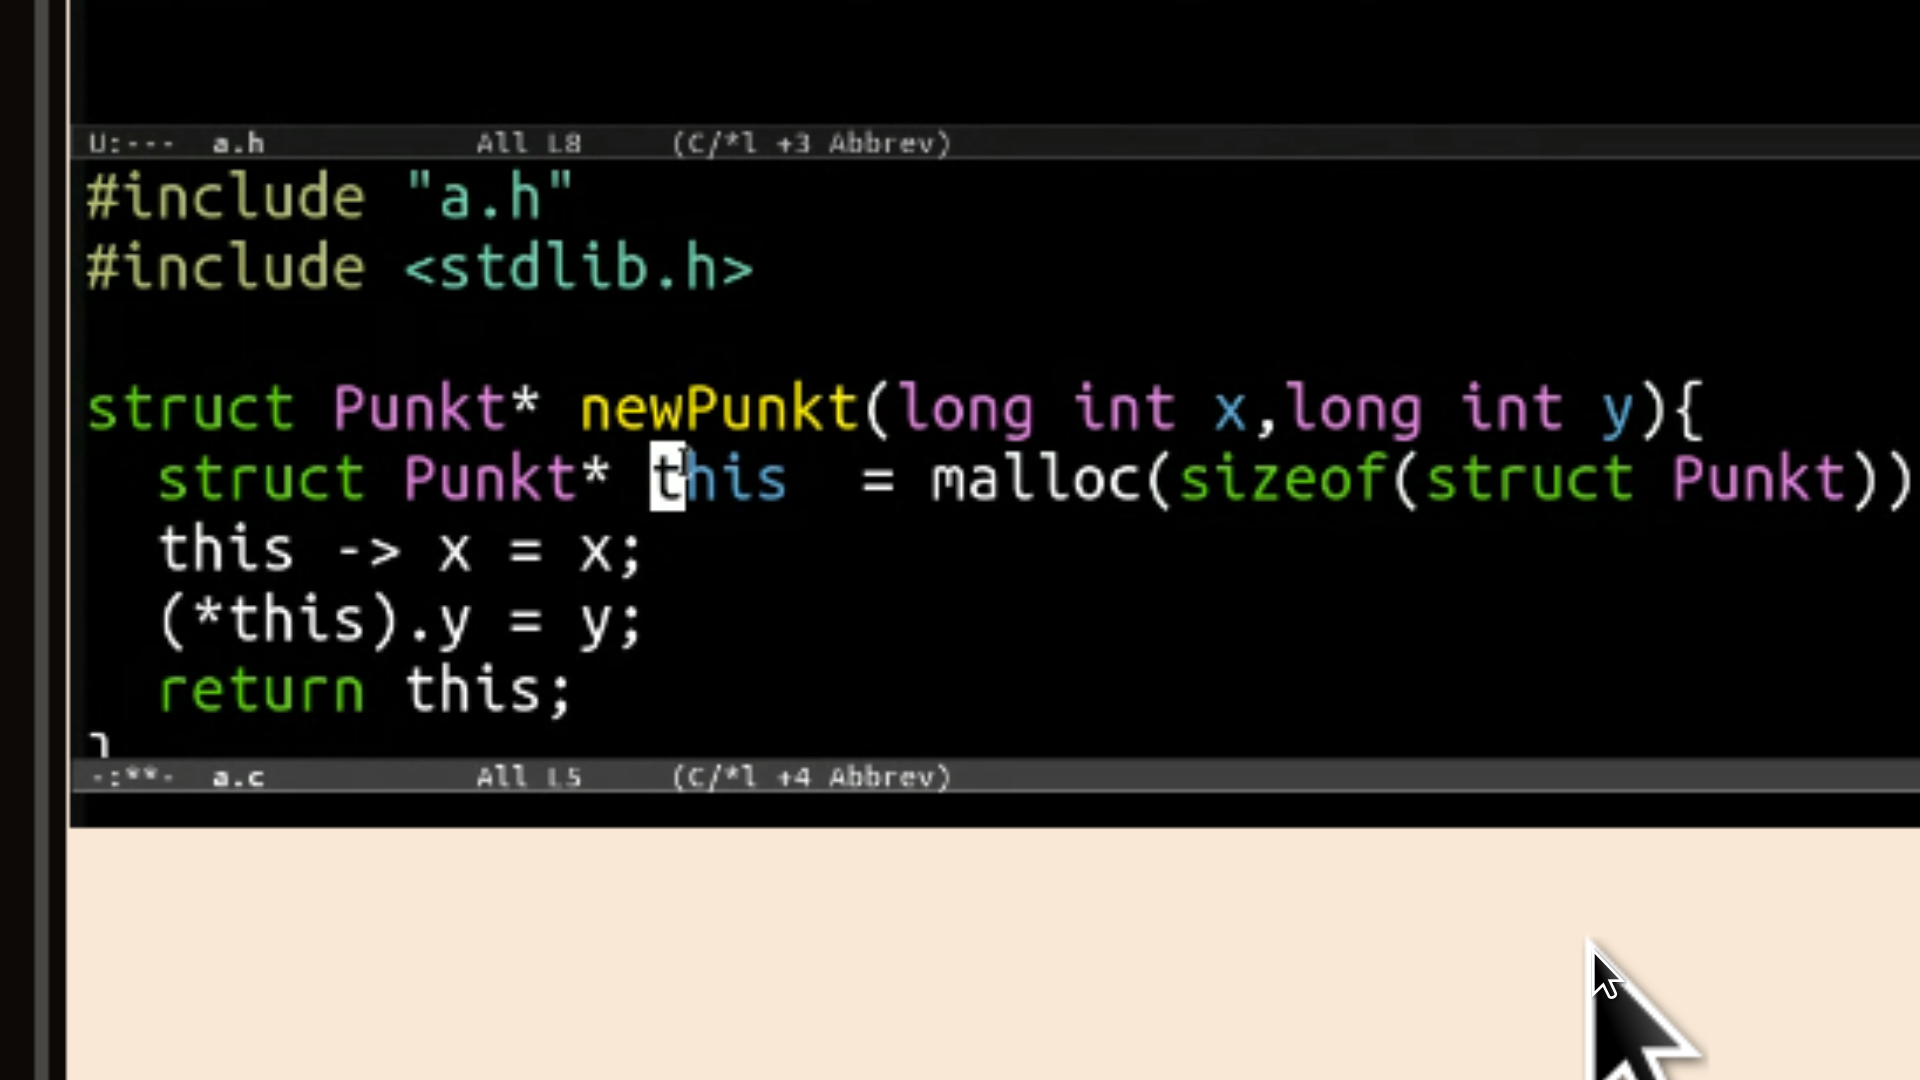
\includegraphics[width=\linewidth]{ckonsample} \\
 	inkludiert werden nur .h Dateien. \\
 	free für das Freigeben von malloc nicht vergessen. \\
 	\subsection*{21.06.2021}
 	Structs Strings \\
 	Typ Synonyme \\
 	typedef int itzelbritzel \\
 	Garbidge Collection \\
 	malloc und free invalid pointer beachten \\
 	\subsection*{24.06.2021}
 	C und Speicher \\
 	Heap, Programmspeicher, Stack, constantspace \\
 	Diese Bereiche müssen uns drum kümmern, macht ja sons keiner!! \\
 	Arbeiten mit Programmen im Programmstore \\
 	Neuer Datentyp \\
 	Enum Aufzählung \\
 	Für ist Enum Wochentag nur eine List von 1 bis 6. C lässt auch andere Zahlen zu. Schweinerei!!
 	Keine Lambda aber Funktionen höherer Ordnung
 	ANSI C \\
 	Code nur global kein Lambdaausdruck \\
 	\subsection*{28.06.2021}
 	Summentypen und Object in C \\
 	Typen beschreiben Mengen von Daten \\
 	union vereinigt typen realisiert Vereinigungsmenge  \\
 	product vereinigt typen ebenfalls realisiert Kreuzprodukt \\
 	Object ist eine Referenz auf dem Stack in den Heap auf entsprechende Nutzdaten. \\
 	\subsection*{01.07.2021}
 	Übersicht über Operatoren in C \\
 	GoTo \\
 	IO \\
 	entweder unär, binär ternär \\
 	pre-, in- oder postfix \\
 	Zuweisungen wie in Jaya \\
 	+=, -=, *= etc. \\
 	Dekrementierung und Dekrementierung gleich wie in Java \\
 	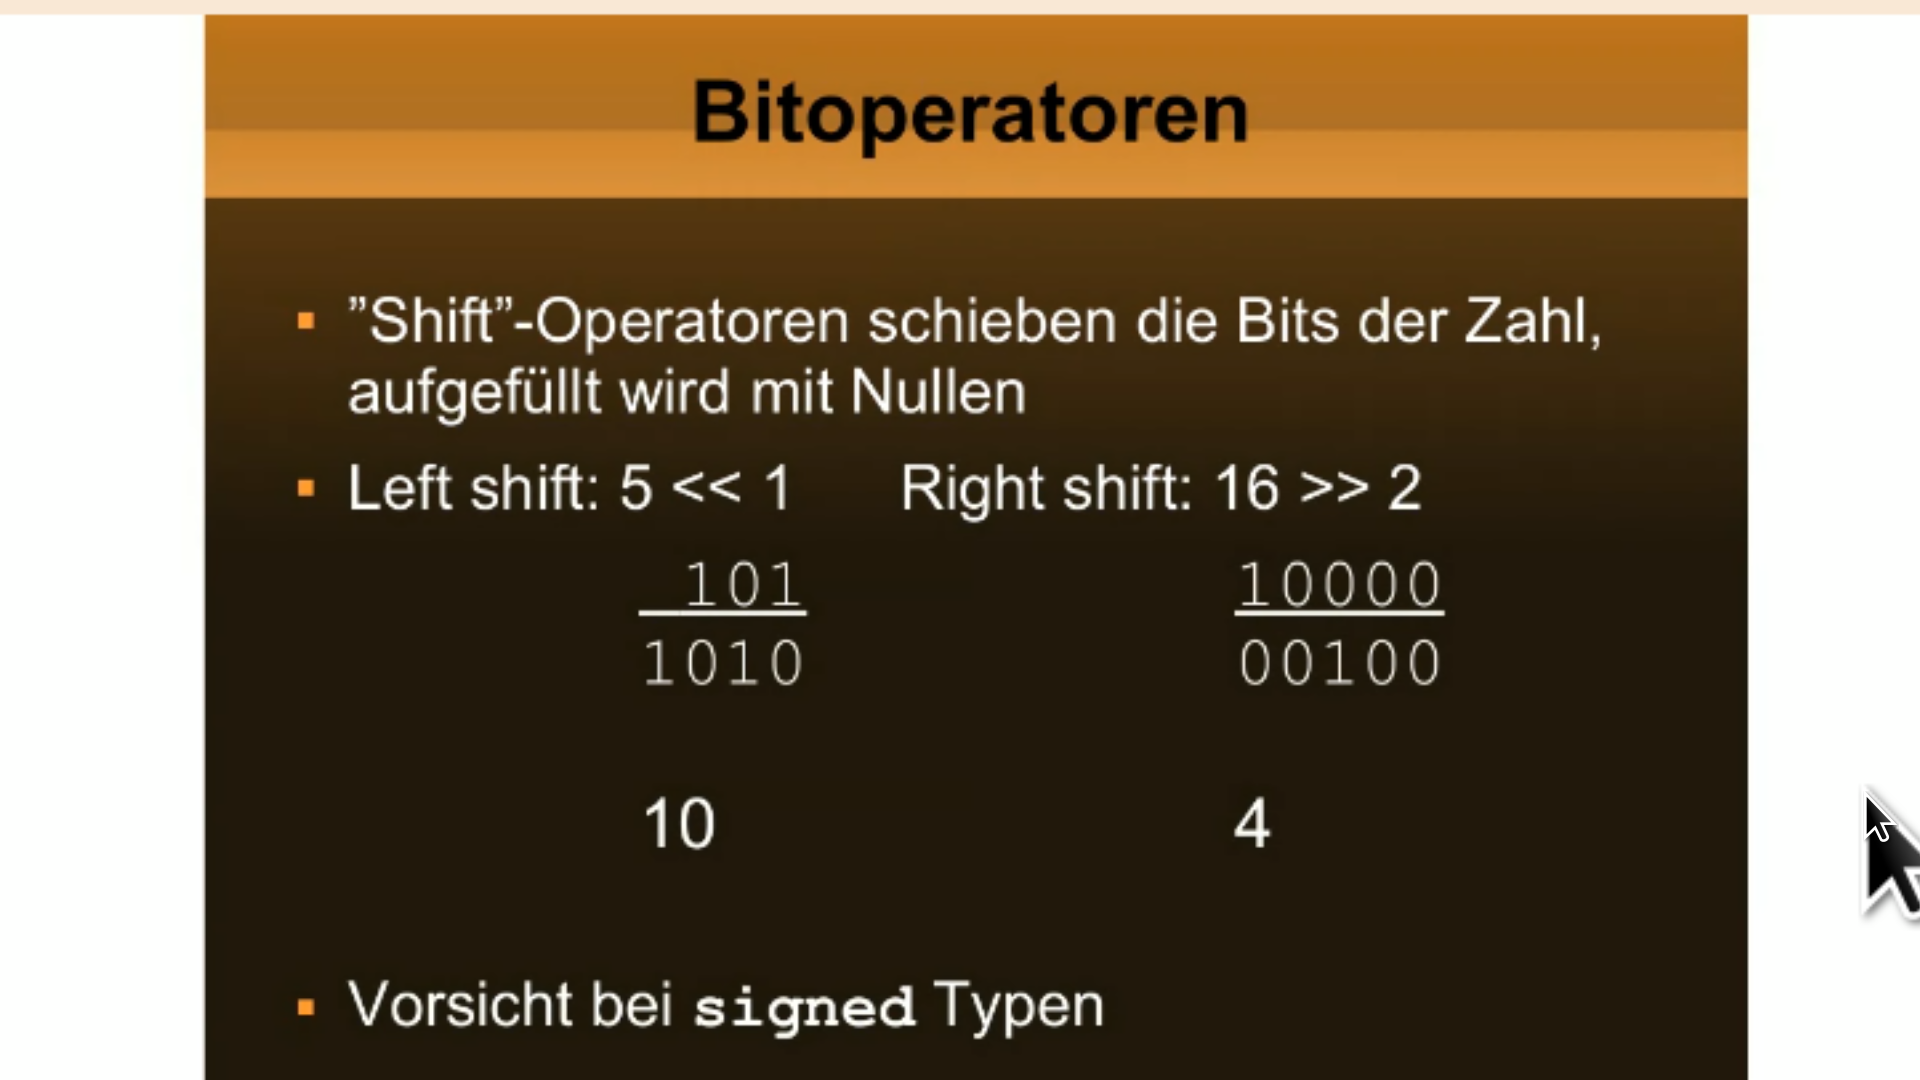
\includegraphics[width=\linewidth]{bitfly}
 	\\
 	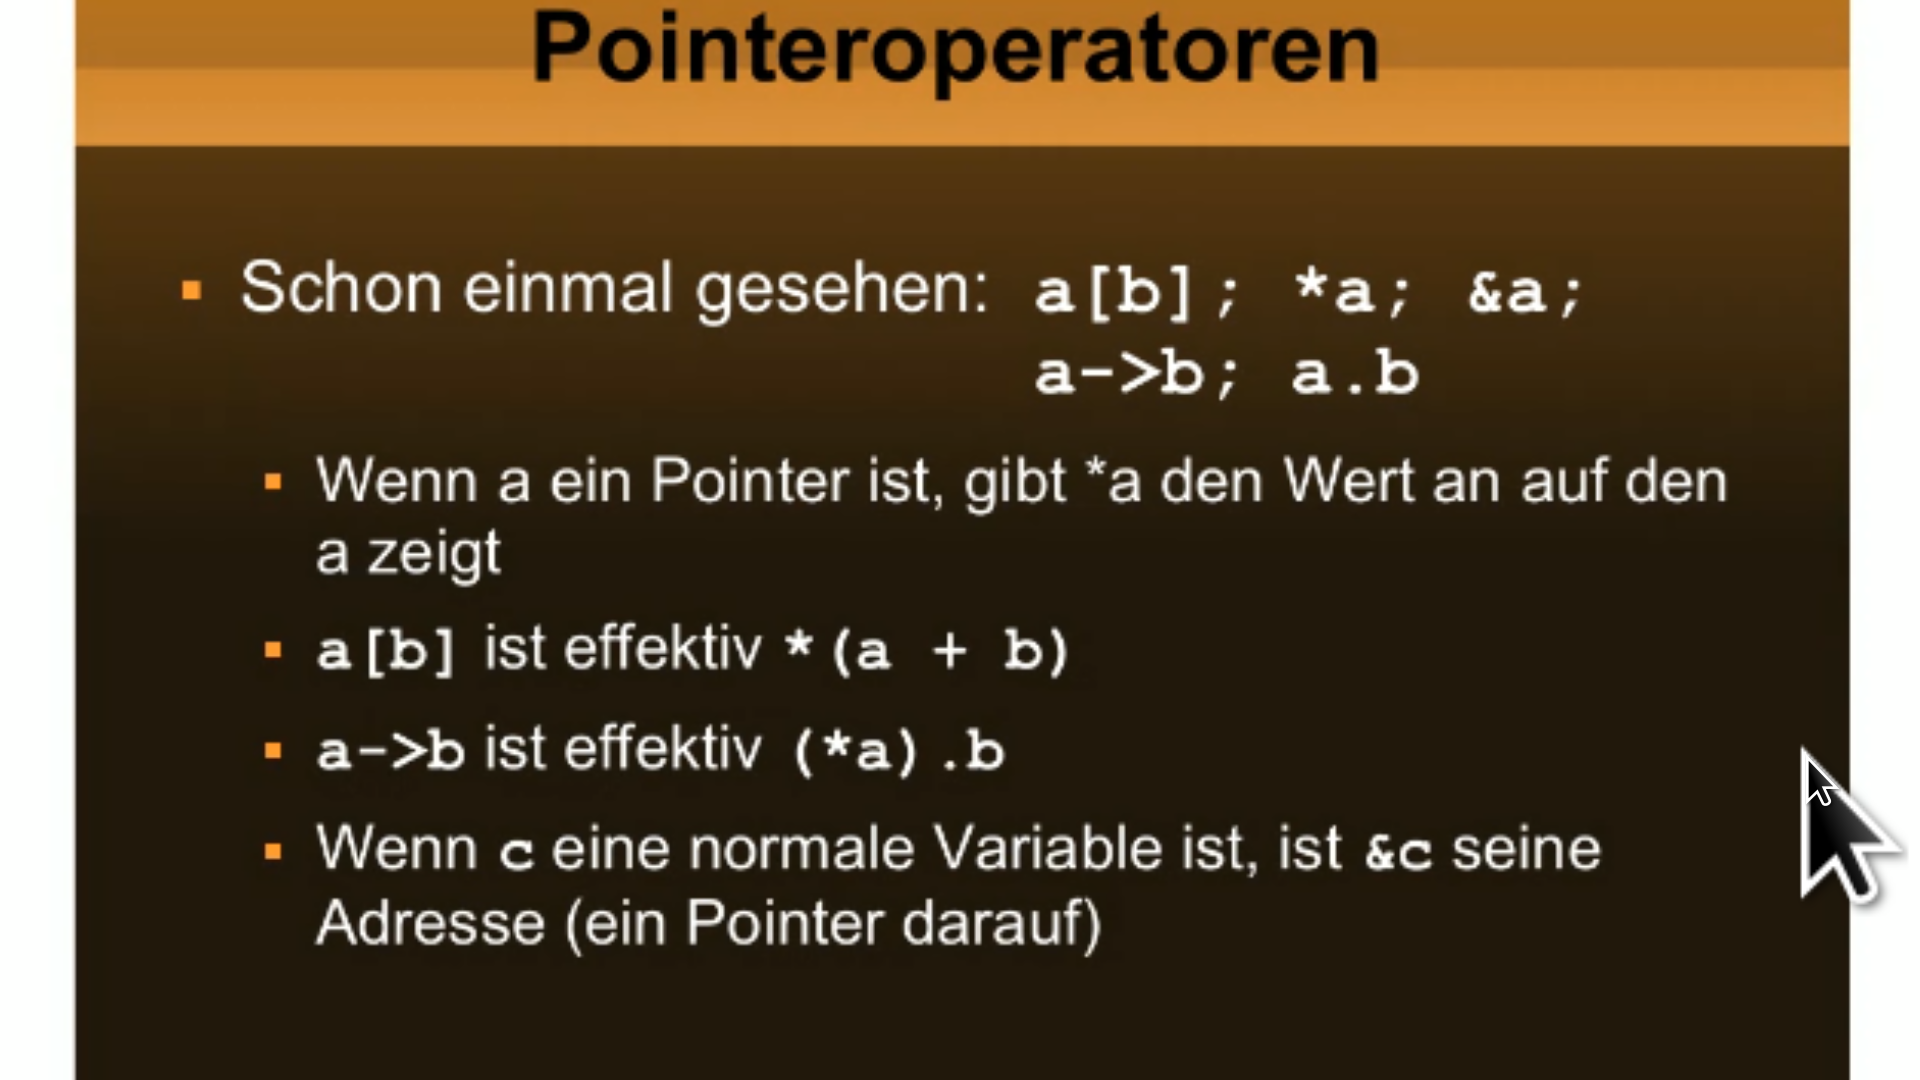
\includegraphics[width=\linewidth]{point} \\
 	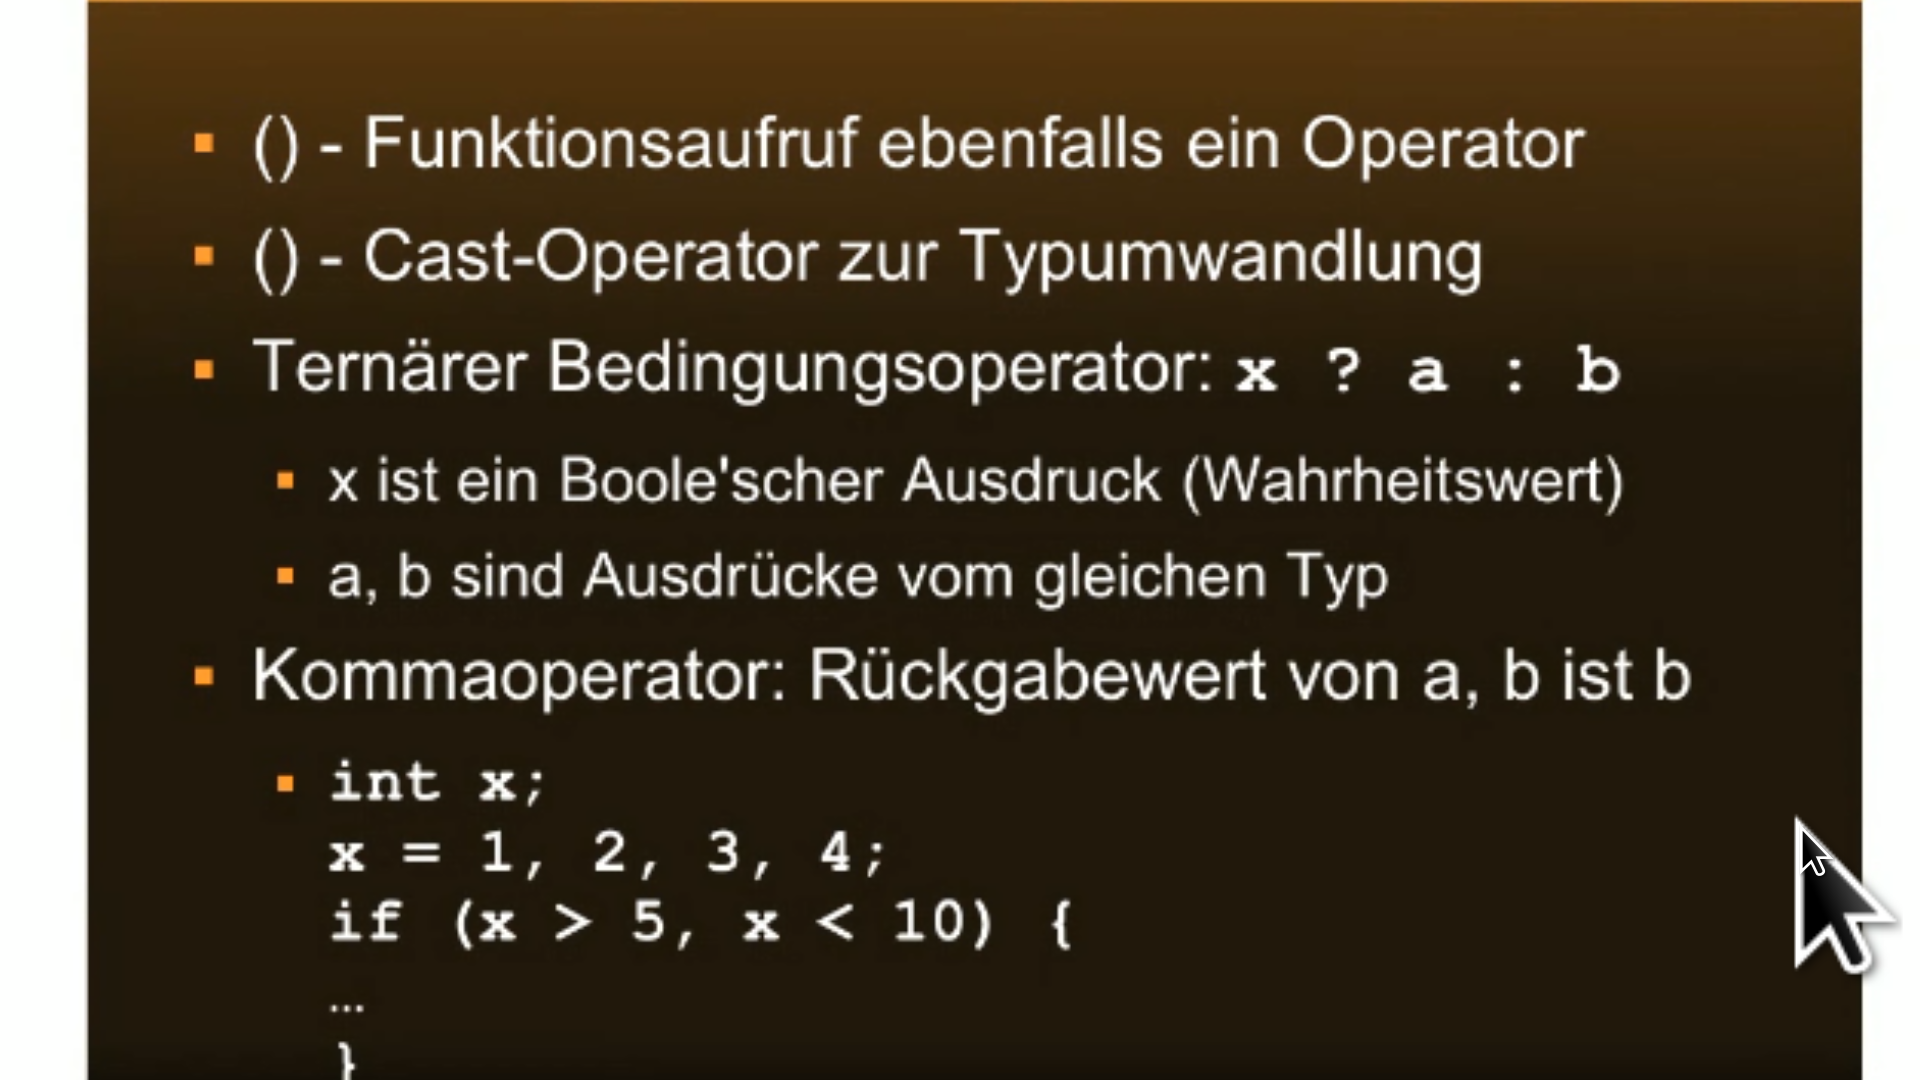
\includegraphics[width=\linewidth]{komma} \\ \\
 	sizeof ist Operator in C \\
 	Beachte Präzedenzen in C \\
 	sizeof kann für die Länge eines Arrays nicht verwendet werden. \\
 	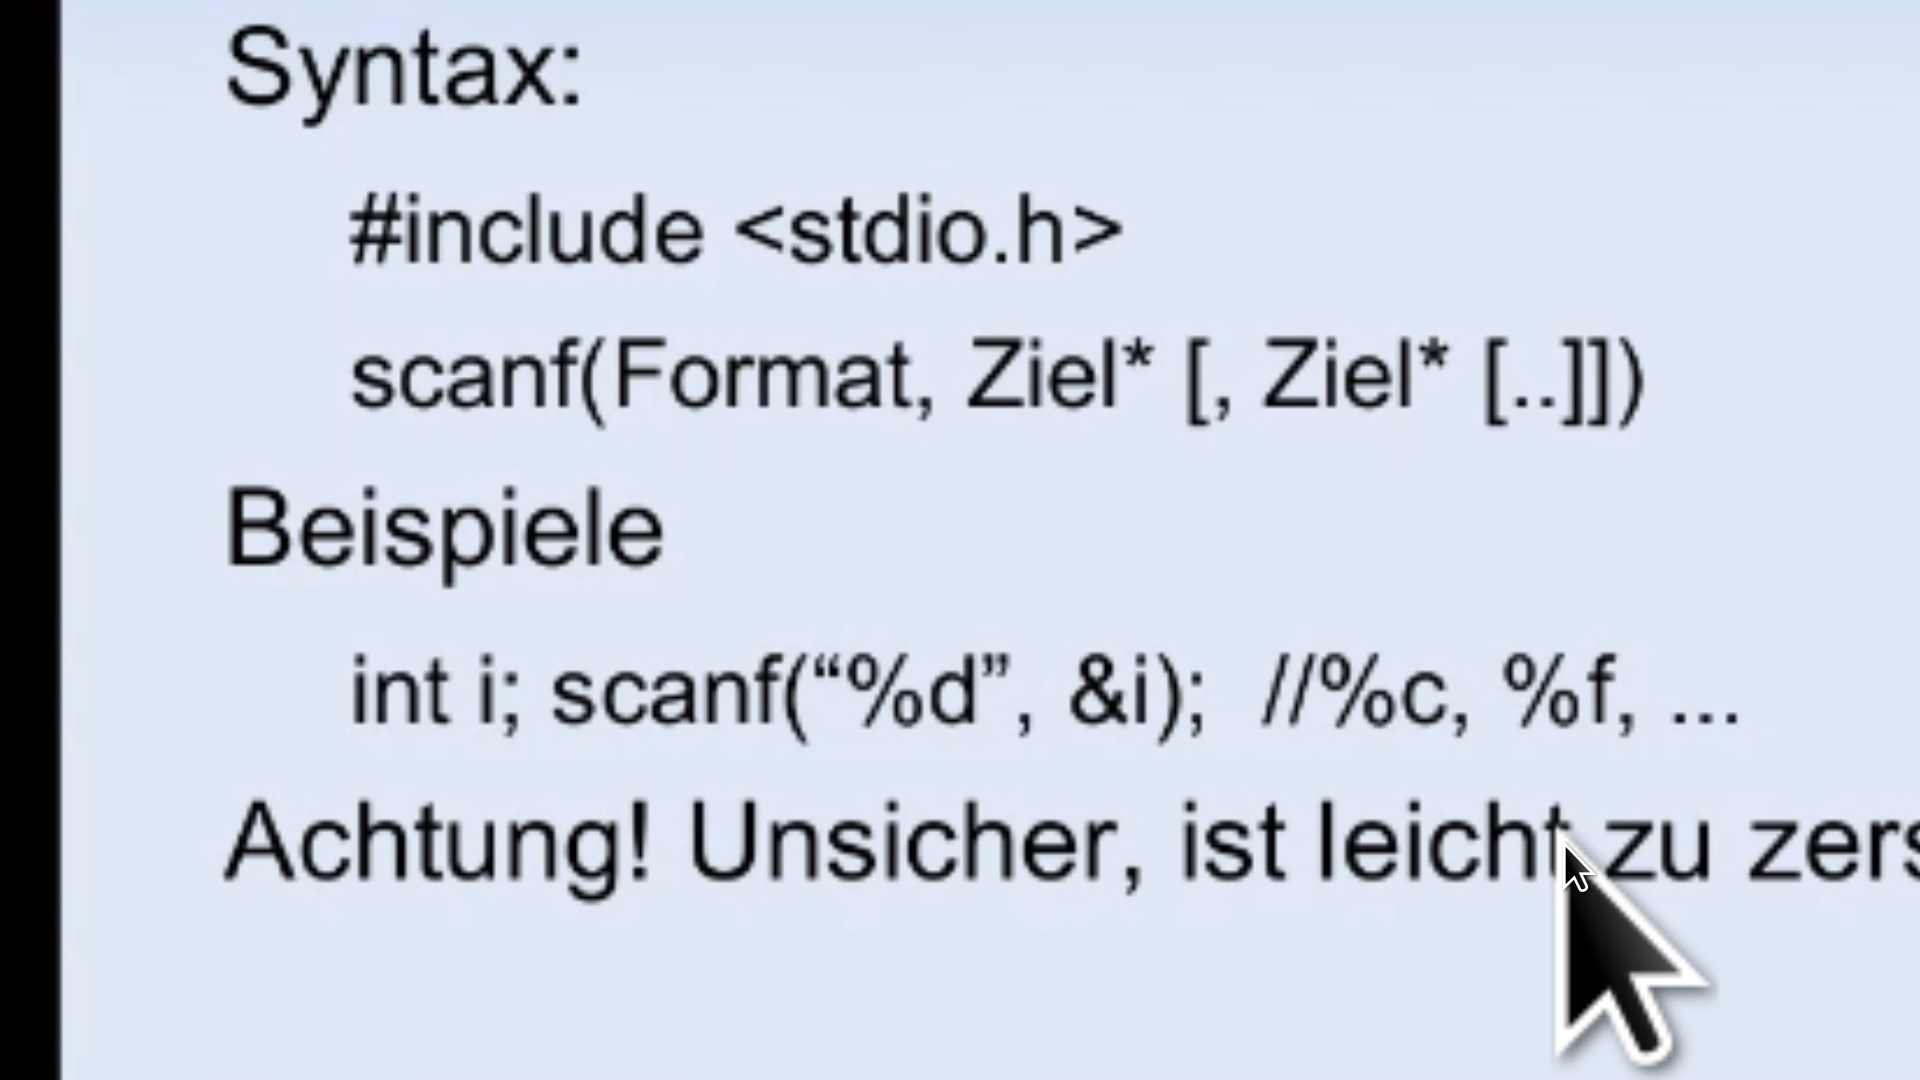
\includegraphics[width=\linewidth]{scanf} \\
	File I/O \\
	
\end{document}